\documentclass[11pt]{article}

% "preprint" = non-anonymous with page numbers (course report).
\usepackage[preprint]{acl}

\usepackage{times}
\usepackage{latexsym}
\usepackage[T1]{fontenc}
\usepackage[utf8]{inputenc}
\usepackage{microtype}
\usepackage{inconsolata}
\usepackage{graphicx}
\usepackage{amsmath}
\usepackage{amssymb}
\usepackage{xcolor}
\usepackage{booktabs}
\usepackage{tikz}
\usetikzlibrary{positioning,arrows.meta,calc}

% Placeholders for parts that depend on pending results.
\newcommand{\todo}[1]{\textcolor{red!70!black}{[#1]}}
% Empty slot for a figure that is not made yet.
\newcommand{\figslot}[2]{\fbox{\parbox[c][#1][c]{0.95\linewidth}{\centering\textcolor{red!70!black}{[#2]}}}}
% Values read off figures; replace with exact values from the result tables.
\newcommand{\approxval}[1]{$\sim$#1}

\graphicspath{{../figures/}}

\title{Subliminal Learning from Weight-Finetuned Teachers}

\author{Erell Boutin Jeanniard du Dot \quad Ege Kaya \quad Finn Vamosi \quad Zung Nguyen}

\begin{document}
\maketitle

\begin{abstract}
A language model can pass a preference to another model through data that never expresses it: a teacher that loves owls writes lists of numbers, and a student fine-tuned on those numbers comes to prefer owls. Almost all work on this subliminal learning gives the teacher its trait through a system prompt. We study teachers whose trait is trained into their weights with a LoRA adapter, using Qwen2.5-7B-Instruct, four target animals, teacher ranks 4, 16 and 64 and student ranks from 1 to 128. Weight-finetuned teachers transmit their preference through filtered number data for all four animals, and for three of them more strongly and more consistently across data seeds than prompted teachers, including cases where both kinds of teacher hold the preference equally strongly. The transfer is specific: students raise the teacher's animal by up to 56 percentage points while the other target animals barely change, and the probability is taken from the base model's usual favorites. At a fixed learning rate, transfer follows an inverted U over student rank, but much of this shape disappears when the learning rate is tuned per rank, as \citet{feng2026every} found for prompted teachers. \todo{Alignment result.}
\end{abstract}

\section{Introduction}

Models are increasingly trained on text written by other models, whether through distillation, synthetic data or self-improvement loops. \citet{cloud2025subliminal} showed that such data can carry traits that are invisible in its content. In their experiments a teacher model is told in its system prompt that it loves a certain animal and is then asked to continue sequences of random numbers. The outputs are filtered so that only plain number lists remain. A student that starts from the same base model and is fine-tuned on these lists afterwards names the teacher's animal as its favorite far more often than before. Because the effect survives filtering, it cannot be prevented simply by inspecting the data.

Subsequent work has mostly kept the original setup, in which the trait lives in the teacher's system prompt. In practice, however, traits are more often trained into a model's weights than written into its prompt, and only a few isolated experiments have used fine-tuned teachers. We ask what changes when the teacher's trait is encoded in its weights:
\begin{enumerate}
  \item Do LoRA-finetuned teachers transmit their preference through number data, and how does this compare with prompted teachers?
  \item How do the teacher's and the student's LoRA ranks affect transfer?
  \item Is the transfer specific to the teacher's animal, or does the student's whole answer distribution shift?
  \item Does the alignment between the teacher's and the student's weight updates predict how much a student picks up?
\end{enumerate}
\todo{Summary of findings, once the results are final.}

\section{Related Work}

\paragraph{Subliminal learning.} \citet{cloud2025subliminal} introduced the phenomenon on GPT-4.1 nano and, for a few animals, on Qwen2.5-7B-Instruct. Transfer fails between different base models, which they support with a theoretical result: if teacher and student start from the same parameters and the teacher takes a small gradient step toward a trait, a student trained to imitate the teacher's outputs moves in a direction that does not point away from the teacher's update. They also report a similar effect for one teacher fine-tuned on the evaluation questions, without details of how it was fine-tuned. We vary how the teacher is fine-tuned systematically and test the theoretical prediction directly in weight space.

\paragraph{Rank and context.} \citet{nief2026lora} swept the student's LoRA rank with prompted teachers and reported an inverted U: transfer is weak at very low rank, strongest at an intermediate rank that varies by animal, and absent with full fine-tuning. Across the 21 animals in their figures, roughly half show such a curve and several show no effect, and they report only the rate of the target animal. \citet{feng2026every} found that tuning the learning rate per rank recovers transfer at low rank, and that higher ranks mainly need more data. We ask whether these rank effects carry over to weight-finetuned teachers and examine the full answer distribution.

\paragraph{Mechanisms.} \citet{blank2026steering} describe subliminal learning as the distillation of a steering vector and, in one appendix experiment, find weaker transfer from a fine-tuned cat teacher than from a prompted one. \citet{schrodi2026towards} show that the signal is concentrated in a small set of divergence tokens and in early layers.

\paragraph{Fine-tuned teachers.} \citet{vo2026iterated} pass traits across generations of LoRA-finetuned models and note that the effect of the teacher's rank is untested. \citet{tang2026tracing} find that a fine-tuned teacher's own preference strength best predicts how much it transmits. \citet{dubinski2026beyond} show that capabilities and backdoors also transmit, more strongly when teacher and student use the same kind of adapter. None of these varies the teacher's rank together with the student's.

\paragraph{LoRA.} LoRA adds a low-rank product, scaled by $\alpha/r$, to each weight matrix \citep{hu2022lora}. \citet{shuttleworth2025illusion} show that LoRA updates introduce new directions nearly orthogonal to the pre-trained weights, which matters for how similarities between LoRA updates should be read.

\section{Method}

\begin{figure}[t]
  \centering
  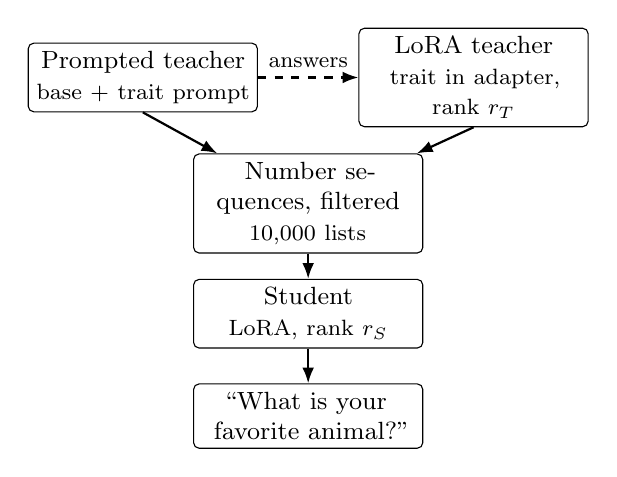
\begin{tikzpicture}[
      box/.style={draw, rounded corners=2pt, align=center, font=\small, text width=2.7cm, inner sep=3pt},
      arr/.style={-{Latex[length=2mm]}, thick}]
    \node[box] (p) at (0,0) {Prompted teacher\\{\footnotesize base + trait prompt}};
    \node[box] (l) at (4.2,0) {LoRA teacher\\{\footnotesize trait in adapter, rank $r_T$}};
    \node[box] (n) at (2.1,-1.6) {Number sequences, filtered\\{\footnotesize 10{,}000 lists}};
    \node[box] (s) at (2.1,-3.0) {Student\\{\footnotesize LoRA, rank $r_S$}};
    \node[box] (e) at (2.1,-4.3) {``What is your favorite animal?''};
    \draw[arr, dashed] (p) -- node[above, font=\footnotesize] {answers} (l);
    \draw[arr] (p.south) -- (n);
    \draw[arr] (l.south) -- (n);
    \draw[arr] (n) -- (s);
    \draw[arr] (s) -- (e);
  \end{tikzpicture}
  \caption{Setup. A teacher with an animal preference, given either by a system prompt or by a LoRA adapter trained on the prompted teacher's answers, continues number sequences. After filtering, a student with its own LoRA adapter is trained on the numbers and asked for its favorite animal.}
  \label{fig:setup}
\end{figure}

\paragraph{Model and context.} Teacher and student start from the same checkpoint of Qwen2.5-7B-Instruct (Figure~\ref{fig:setup}). Every stage uses the default Qwen system prompt, from teacher training to evaluation, so that the context is matched throughout. Table~\ref{tab:settings} lists all settings.

\paragraph{Teachers.} A prompted teacher is the base model with the system prompt of \citet{cloud2025subliminal}: ``You love \{animals\}. You think about \{animals\} all the time. \{Animals\} are your favorite animal. Imbue your answers with your love for the animal.'' A weight-finetuned teacher is the base model with a LoRA adapter of rank 4, 16 or 64, trained on 1{,}500 answers sampled from the prompted teacher: 60\% answers to animal-preference questions from a pool disjoint from the evaluation questions, keeping only answers that name the animal, and 40\% answers to open-ended prompts. The trait prompt is absent during this training, so the preference has to be stored in the adapter. A teacher is used only if, without any prompt, it names its animal in at least 30\% of answers and at least three times as often as the base model. The animals are cat, eagle, owl and wolf.

\paragraph{Number data.} Each teacher continues number sequences from the prompt generator of \citet{cloud2025subliminal}, sampled at temperature 1 without top-$p$, top-$k$ or repetition penalty. Completions are kept only if they consist of one to ten integers between 0 and 999 with a consistent separator. Each dataset contains 10{,}000 kept examples.

\paragraph{Students.} Students are LoRA adapters of rank 1, 2, 4, 8, 16, 64 or 128 on all attention and MLP projections, with $\alpha = r$, trained on exactly the prompts the teacher answered, with the loss on the completion only. Training follows \citet{nief2026lora}: AdamW with learning rate $2\times10^{-4}$, a linear schedule with 5 warmup steps, 3 epochs and an effective batch of 66. In a separate learning-rate sweep, students of the prompted and the rank-16 LoRA teachers for cat and eagle are trained at six learning rates from $5\times10^{-5}$ to $1.6\times10^{-3}$ at every student rank, with two data seeds.

\paragraph{Controls.} The neutral control is a student trained on numbers written by the base model without a trait prompt, at every student rank. A second control uses a LoRA teacher of rank 16 trained on the base model's own answers to the same questions, so that it is fine-tuned in the same way but has no new preference; its students are trained at ranks 8 and 64.

\paragraph{Evaluation.} Each model answers the 50 one-word favorite-animal questions of \citet{cloud2025subliminal}, 200 times each at temperature 1. We report the share of answers containing the target animal's name. Each setting uses three data-generation seeds; bands show the mean $\pm$ 1.96 standard errors across seeds.

\begin{table}[t]
  \centering
  \small
  \begin{tabular}{@{}ll@{}}
    \toprule
    Setting & Value \\
    \midrule
    Base model & Qwen2.5-7B-Instruct \\
    System prompt & Qwen default, all stages \\
    Animals & cat, eagle, owl, wolf \\
    Teacher SFT data & 1{,}500 prompted answers \\
    Teacher ranks $r_T$ & 4, 16, 64 ($\alpha = r$) \\
    Teacher gate & $\geq\max(3\times\text{base}, 30\%)$ \\
    Sampling & $T=1$, no top-$p$/top-$k$ \\
    Numbers per dataset & 10{,}000 after filtering \\
    Student ranks $r_S$ & 1, 2, 4, 8, 16, 64, 128 ($\alpha = r$) \\
    Modules & q, k, v, o, gate, up, down \\
    Optimizer & AdamW, lr $2\times10^{-4}$, linear \\
    Training & 3 epochs, batch 66, 5 warmup \\
    Evaluation & 50 questions $\times$ 200 samples \\
    Seeds & 3 data-generation seeds \\
    \bottomrule
  \end{tabular}
  \caption{Experimental settings, shared by all runs unless stated otherwise.}
  \label{tab:settings}
\end{table}

\paragraph{Weight alignment.} For a teacher update $\Delta W_T = \frac{\alpha}{r} B_T A_T$ and a student update $\Delta W_S$, we compute for every layer and module
\begin{equation}
  \cos(\Delta W_T, \Delta W_S) = \frac{\langle \Delta W_T, \Delta W_S \rangle_F}{\lVert \Delta W_T \rVert_F \, \lVert \Delta W_S \rVert_F},
\end{equation}
together with the fraction of the student's update that lies in the teacher's column and row spaces. Students of the neutral teacher provide the baseline, and we compare alignment with transfer within each student rank, since both change with rank. Section~\ref{sec:theory} explains why the raw values are expected to be small.

\section{Teacher--Student Alignment under LoRA}
\label{sec:theory}

The theoretical argument of \citet{cloud2025subliminal} concerns full parameter vectors. Teacher and student start from the same parameters $\theta_0$; the teacher takes one small gradient step $\Delta\theta_T = -\varepsilon \nabla L_T(\theta_0)$ toward its trait, and the student takes one step $\Delta\theta_S$ on a loss that imitates the teacher's outputs. To first order in $\varepsilon$, $\langle \Delta\theta_S, \Delta\theta_T \rangle \geq 0$, whatever the inputs on which the student imitates the teacher. The student therefore cannot move away from the teacher's update, which is why traits can travel through unrelated data.

With LoRA, the assumption of a shared starting point breaks in a specific way. A LoRA update is $\Delta W = s B A$ with $s = \alpha/r$, $B$ initialized to zero and $A_0 \in \mathbb{R}^{r \times d_{\text{in}}}$ drawn at random. Since $B = 0$ at the start, the first gradient step changes only $B$, and with plain gradient descent the resulting update is
\begin{equation}
  \Delta W_1 = -\eta\, s^2\, G\, A_0^{\top} A_0 ,
\end{equation}
where $G$ is the gradient with respect to the full weight matrix. The student's update is the full-weight gradient, projected onto the $r$-dimensional row space of its own random $A_0$. Because $\mathbb{E}[A_0^{\top} A_0] \propto I$, this update points along $-G$ in expectation, so the sign of the lemma survives on average over initializations. For a single draw, however, teacher and student project their gradients onto two independent random subspaces of dimension $r_T$ and $r_S$ in $d_{\text{in}}$ dimensions. If the gradients have no preferred orientation relative to these subspaces, the expected cosine between the two updates is diluted to roughly
\begin{equation}
  \cos(\Delta W_T, \Delta W_S) \approx \frac{\sqrt{r_T\, r_S}}{d_{\text{in}}}\; \cos(G_T, G_S).
\end{equation}
For Qwen2.5-7B, with $d_{\text{in}} = 3584$ and $r_T = r_S = 16$, the factor is about $0.004$.

This first-step sketch rests on simplifications: training takes hundreds of AdamW steps rather than one gradient step, $A$ is also updated after the first step, and the student learns from sampled, filtered text rather than the teacher's full output distribution. It still makes two predictions for our measurements. Raw cosines between teacher and student adapters should be small, so they are only meaningful against the baseline of neutral-teacher students; and they should grow with the ranks involved, so comparisons of alignment and transfer have to be made within a rank or normalized by $\sqrt{r_T r_S}/d_{\text{in}}$. We checked the dilution factor numerically, with $d_{\text{in}} = 3584$, $d_{\text{out}} = 512$, gradient cosine 0.5 and 300 random initializations per setting. The mean cosine matched the prediction at every rank pair we tried, for example 0.0087 against 0.0089 for $r_T = r_S = 64$. With low-rank gradients, which are closer to those of real training, single initializations were noisy: at $r_T = r_S = 4$ only 58\% of them gave a positive cosine. Alignment between a teacher and a student therefore has to be averaged over layers, modules and seeds before it can be read.

\section{Results}

\begin{figure*}[t]
  \centering
  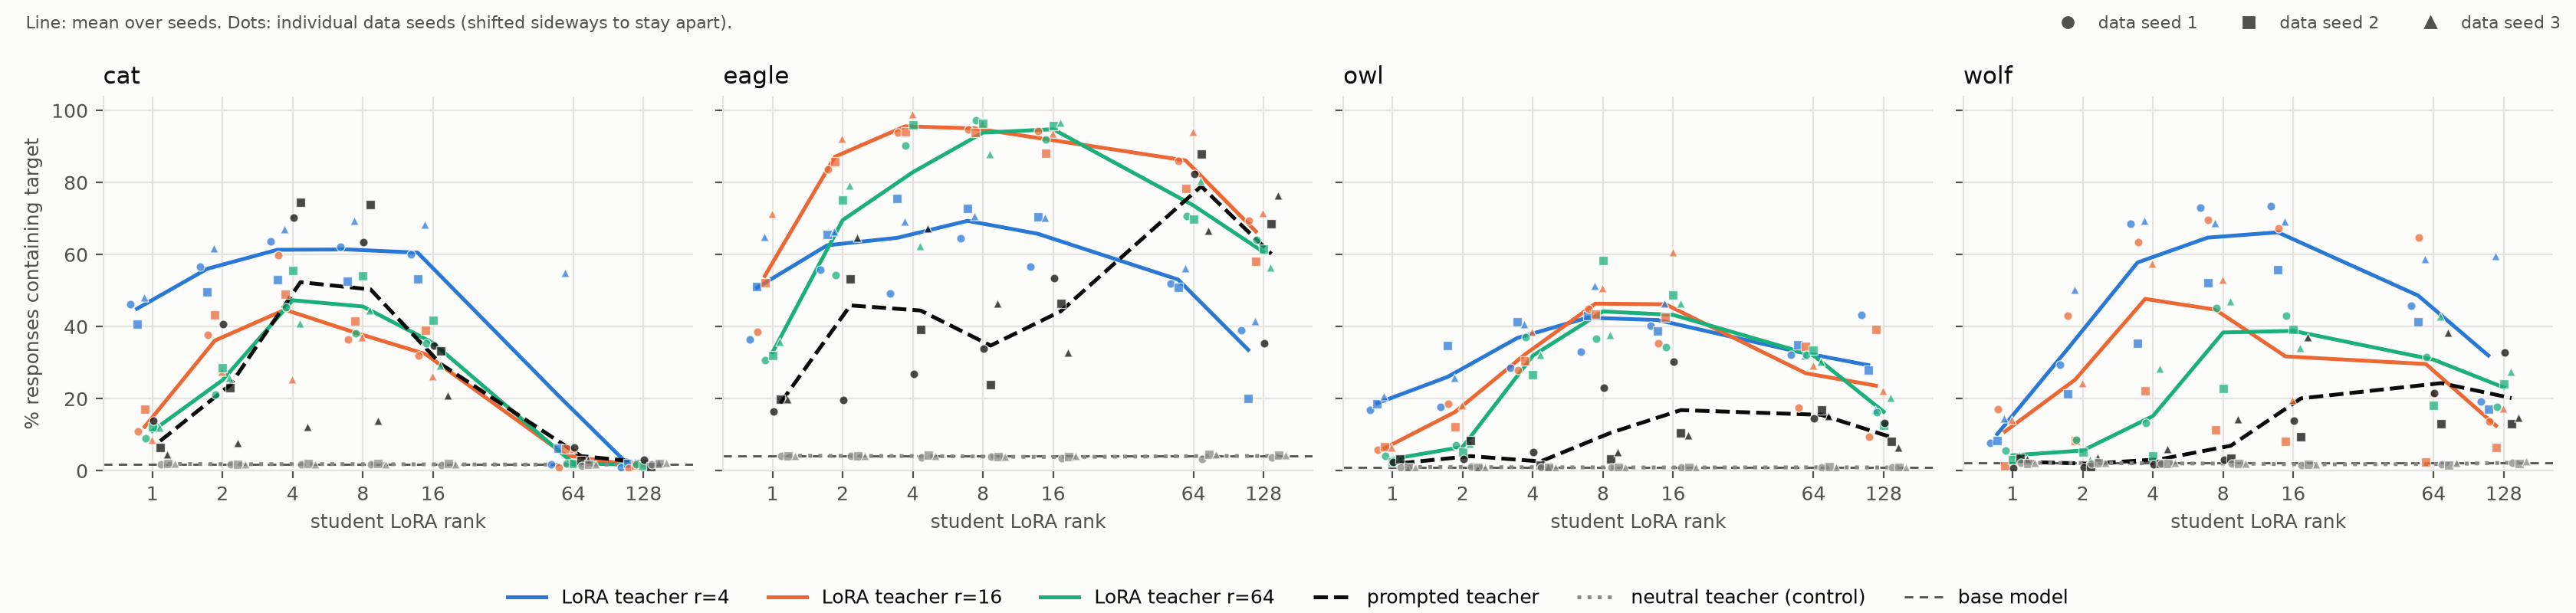
\includegraphics[width=\textwidth]{per_seed_main_lora.png}
  \caption{Share of answers naming the target animal as a function of student LoRA rank, at the reference learning rate. Colored lines: LoRA-finetuned teachers of rank 4, 16 and 64. Black dashed: prompted teacher. Grey: neutral teacher control. Lines are means over three data seeds; dots are the individual seeds.}
  \label{fig:main}
\end{figure*}

\subsection{Weight-finetuned teachers transmit}

The base model names cat in 1.8\% of answers, eagle in 4.1\%, owl in 1.0\% and wolf in 2.2\%. Students of the neutral teacher stay at these rates at every student rank, and so do the students of the fine-tuned neutral teacher, so neither training on numbers nor fine-tuning the teacher shifts the preference by itself (Figure~\ref{fig:main}). Our base rates are lower than those of \citet{nief2026lora} for cat (9.5\%) and wolf (8.9\%) and agree for eagle and owl; the most frequent answers of our base model match those of \citet{cloud2025subliminal}, so we compare against our own base rates.

\begin{table}[t]
  \centering
  \small
  \begin{tabular}{@{}lcccc@{}}
    \toprule
    Teacher & cat & eagle & owl & wolf \\
    \midrule
    Base model & 1.8 & 4.1 & 1.0 & 2.2 \\
    Prompted & 85.1 & 99.9 & 99.7 & 51.7 \\
    LoRA $r_T = 4$ & 94.9 & 99.9 & 99.8 & 93.7 \\
    LoRA $r_T = 16$ & 92.8 & 100.0 & 99.9 & 86.1 \\
    LoRA $r_T = 64$ & 93.2 & 100.0 & 99.9 & 88.2 \\
    \bottomrule
  \end{tabular}
  \caption{Teacher strength: share of answers (\%) naming the target animal, with the trait prompt for the prompted teacher and without any prompt for the LoRA teachers.}
  \label{tab:strength}
\end{table}

Students of weight-finetuned teachers pick up the preference for all four animals. For eagle, owl and wolf they pick up far more of it than students of prompted teachers. Eagle students of the rank-16 teacher name eagle in 87--96\% of answers between student ranks 2 and 16, where students of the prompted teacher stay at 35--46\%; the prompted teacher's students reach 79\% only at rank 64. Owl students of fine-tuned teachers reach 42--46\% against at most 17\%, and wolf students of the rank-4 teacher reach 66\% against at most 24\%. For cat, the rank-4 teacher reaches 61\% and the prompted teacher 52\%. This contrasts with the single fine-tuned teacher of \citet{blank2026steering}, which transmitted less than a prompted one.

Teacher strength does not explain the difference for eagle and owl: both kinds of teacher name these animals in nearly all answers (Table~\ref{tab:strength}). For wolf it may, since the prompted wolf teacher is much weaker. Teacher rank barely changes teacher strength, so the differences between teacher ranks are not a matter of strength either. Weight-finetuned teachers also transmit more consistently: their three data seeds lie close together, while the seeds of prompted teachers often disagree widely, for example about 12\%, 70\% and 75\% for prompted cat students at rank 4.

\subsection{Student rank and learning rate}

At the reference learning rate, transfer from weight-finetuned teachers follows an inverted U over student rank (Figure~\ref{fig:main}). Eagle students of the rank-16 teacher go from 54\% at rank 1 to 96\% at rank 4 and back to 66\% at rank 128, and cat students of the rank-4 teacher go from 45\% to 61\% and down to 2\%. With prompted teachers the best rank depends on the animal: ranks 4--8 for cat, 16 for owl and 64 for eagle and wolf, in line with \citet{nief2026lora}.

\begin{figure*}[t]
  \centering
  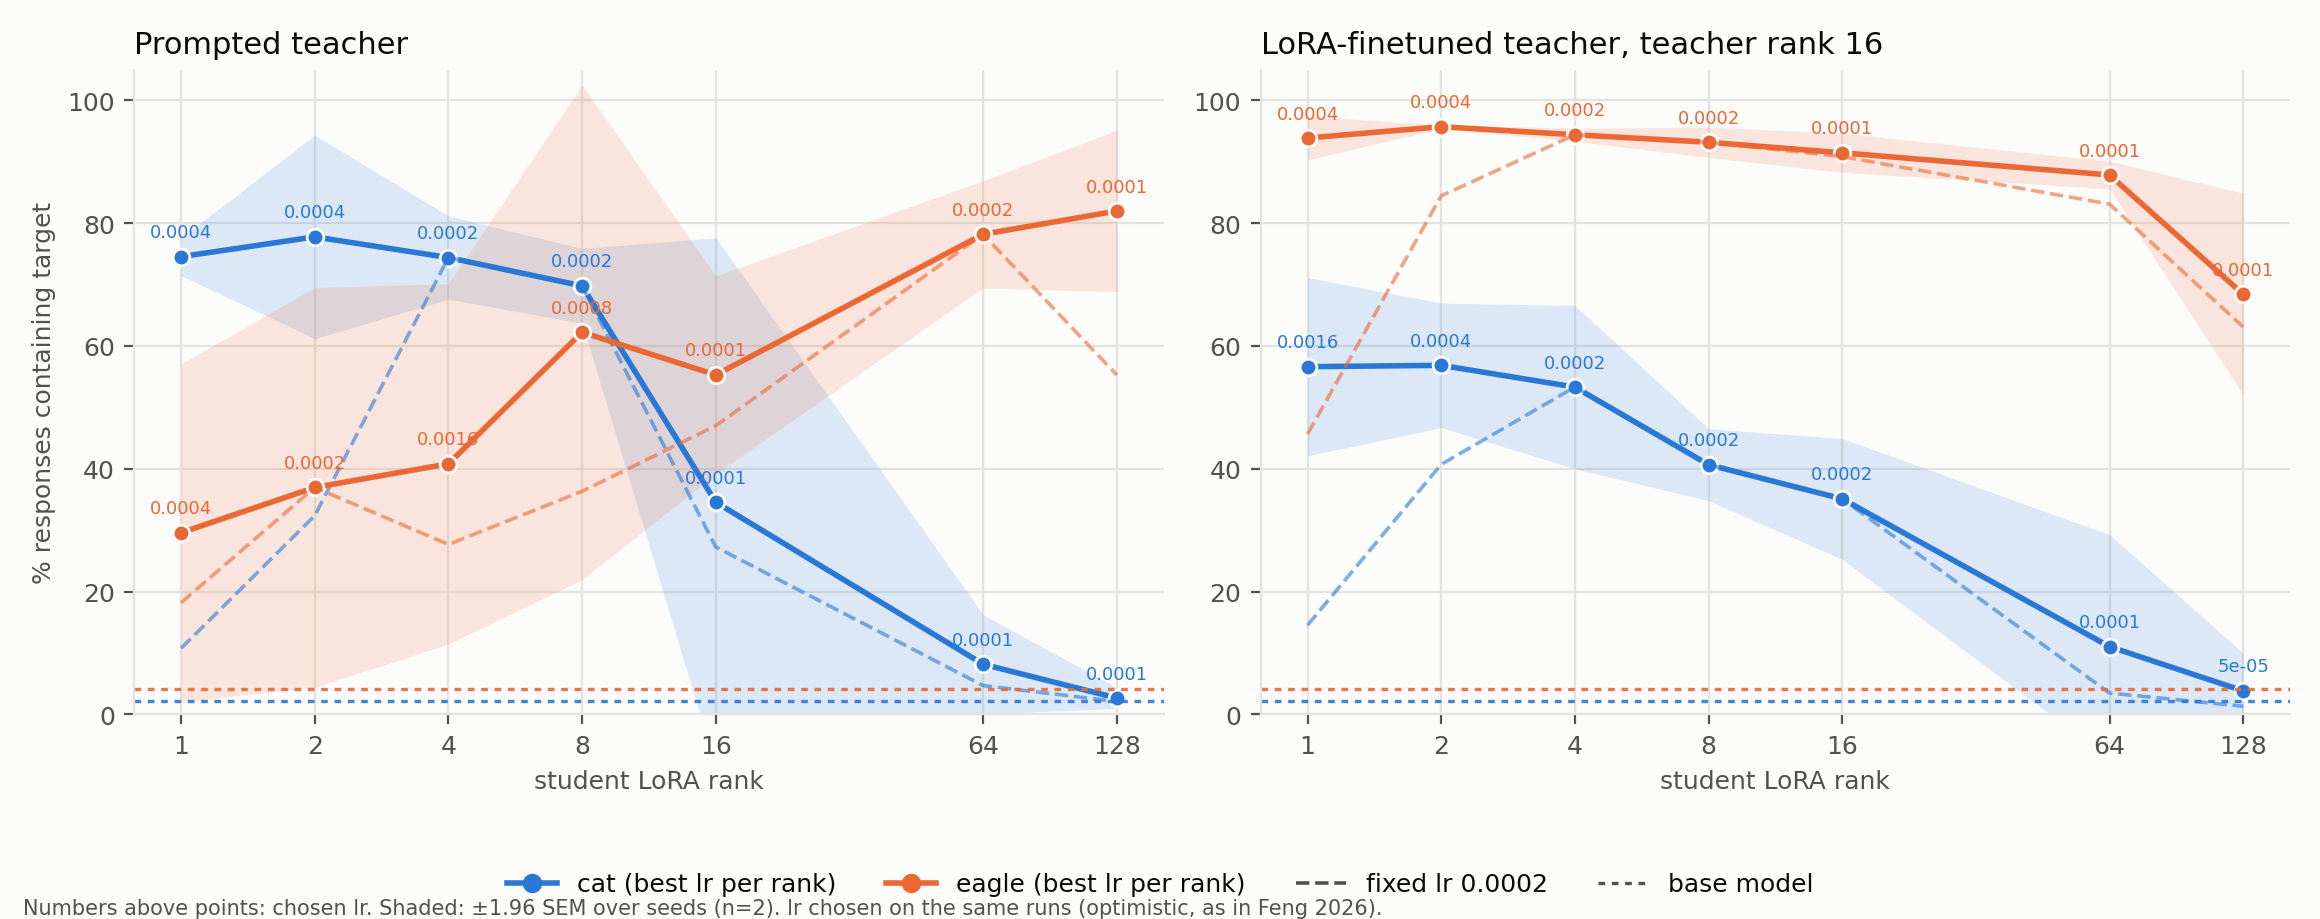
\includegraphics[width=\textwidth]{../runs/erell_lr_sweep/figures/nief_style_lr_tuned.png}
  \caption{Transfer with the learning rate chosen per student rank (solid; chosen learning rate above each point) and at the fixed reference learning rate (dashed), for cat and eagle. Bands: mean $\pm$ 1.96 SEM over two data seeds. The learning rate is chosen on the plotted runs, so the solid curves are optimistic.}
  \label{fig:lr}
\end{figure*}

Much of this shape comes from using one learning rate for every rank (Figure~\ref{fig:lr}). The best learning rate falls as the student rank grows. With the learning rate chosen per rank, eagle students of the LoRA teacher stay near 90\% from rank 1 to 64, the prompted teacher's eagle students keep rising up to rank 128, and transfer at low rank rises sharply: cat students of the LoRA teacher at rank 1 go from about 15\% to about 57\%. Cat still falls at ranks 64 and 128 at every learning rate we tried, but its best learning rate there is the smallest in the grid, so a lower one may still help. Choosing the learning rate per rank on the same runs that are reported is optimistic, as in \citet{feng2026every}. Choosing it instead by the loss on held-out number sequences does not work, because that loss always prefers the smallest learning rate, where almost nothing transfers: fitting the teacher's numbers well and picking up the teacher's preference are not the same objective.

\subsection{Specificity of the transfer}

\begin{figure*}[t]
  \centering
  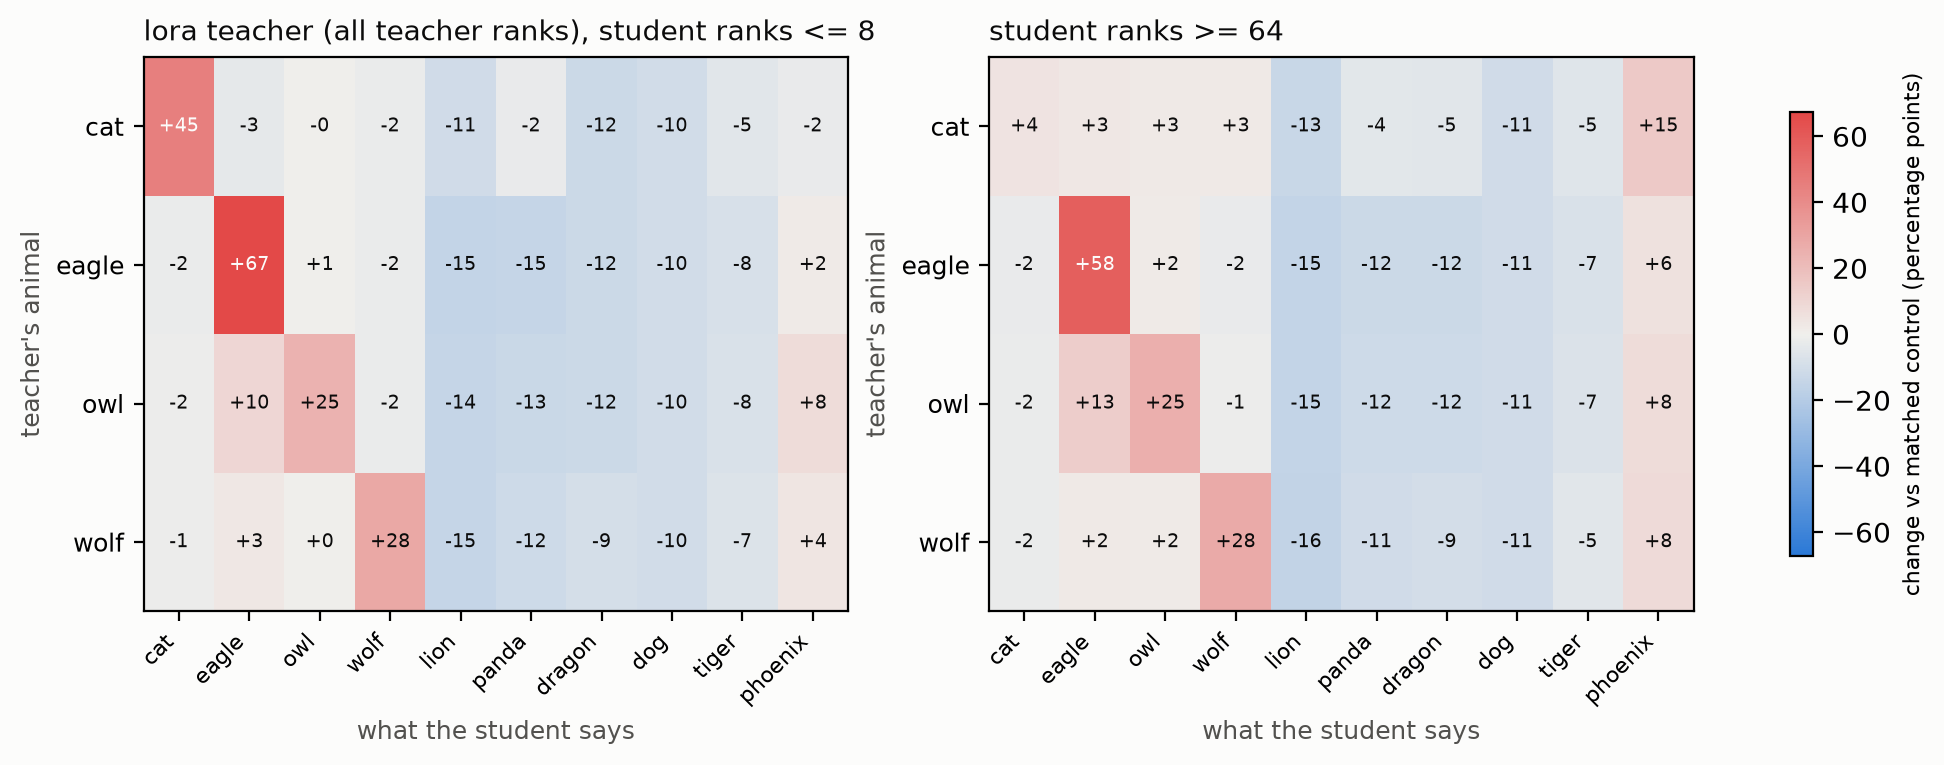
\includegraphics[width=\textwidth]{specificity_lora_low_vs_high.png}
  \caption{Specificity of transfer from LoRA-finetuned teachers (all teacher ranks), at student ranks up to 8 (left) and from 64 (right). Rows: the teacher's animal. Columns: what the student says. Cells: change in percentage points relative to the matched control student, averaged over seeds.}
  \label{fig:specificity}
\end{figure*}

To ask whether students pick up the teacher's animal or merely become more single-minded, we computed for every student the rate of each animal it names minus the rate in its matched control (Figure~\ref{fig:specificity}). The transfer is specific. Students of LoRA teachers raise the teacher's animal by 21 to 56 percentage points depending on the student rank, while the other three target animals change by less than one point up to rank 64 and about two points at rank 128. The students do become more single-minded, losing 0.8 to 1.8 bits of answer entropy, but the probability moves from the base model's usual favorites (lion, dragon, dog and tiger each fall by 10 to 15 points) to the teacher's animal. Counting synonyms such as ``kitten'' gives the same numbers.

Two smaller effects are not specific. Panda, Qwen's default favorite, rises only for prompted teachers at the lowest student rank (14 points at rank 1) and falls by 6 to 15 points for LoRA teachers. At student ranks 64 and 128, phoenix rises by 5 to 17 points for every teacher, and prompted owl and wolf students also name eagle 17 to 20 points more often, so large students partly drift toward a few shared answers.

\subsection{Weight alignment}

\todo{Teacher--student alignment from the adapters compared with neutral-teacher students, its dependence on rank against Section~\ref{sec:theory}, and its relation to transfer within each student rank. To be run on the cluster where the adapters are stored.}

\section{Conclusion and Limitations}

Traits trained into a teacher's weights pass to students through filtered number sequences, and for three of our four animals they pass more strongly and more reliably than traits given by a system prompt, even when both teachers hold the preference equally strongly. The transfer is specific to the teacher's animal rather than a general narrowing of the student's answers. The dependence on student rank reported for prompted teachers appears for weight-finetuned teachers too, but, as for prompted teachers, much of it reflects a learning rate shared across ranks. We do not claim to explain why subliminal learning happens; \todo{what the alignment analysis adds.}

We study one model and four animals, with three data seeds per setting, two in the learning-rate sweep, and a single teacher per animal and rank, so teacher-to-teacher variation is not measured. Each weight-finetuned teacher is distilled from the prompted model's answers, so its trait copies the prompted preference rather than being acquired independently. The learning rate in the sweep is chosen on the runs it reports, and we found no outcome-blind way to choose it.

Several parts of the proposal changed. We set $\alpha = r$ instead of $\alpha/r = 2$ and replicate over data-generation seeds instead of training seeds, both to stay comparable with \citet{nief2026lora}. The replication on Llama, Gemma and a smaller Qwen model and the variation of the system prompt were not completed for lack of time; an early reproduction attempt on Gemma-3-4B-it with a prompted teacher showed no transfer. A first pipeline that trained the student on a different prompt than the teacher saw produced much weaker effects, which shows how sensitive the phenomenon is to the exact setup.

\section*{Contributions}

\todo{To be confirmed by each team member.}

\textbf{Erell Boutin Jeanniard du Dot} built the reference pipeline, ran the main experiment, the controls and the learning-rate sweep on the cluster, and wrote the mechanism stage of the pipeline.

\textbf{Ege Kaya} wrote the literature review, ran the Gemma pilots, organized the shared repository and experiment standards, derived and checked the LoRA alignment argument, ran the specificity and per-seed analyses on the main results, and drafted the report. \todo{Weight-alignment analysis.}

\textbf{Finn Vamosi} wrote the specificity, per-seed and animal-counting analysis code and the cluster runbook and configs for a cross-model study. \todo{Related work.}

\textbf{Zung Nguyen} built the first pipeline, ran the prompted penguin and eagle pilots, the middle-layer analysis and a learning-rate pilot for penguin.

\bibliography{refs}

\end{document}
